\documentclass{llncs}
%\documentclass[letterpaper, 10 pt, conference]{llncs}
%\IEEEoverridecommandlockouts
%\overrideIEEEmargins

\usepackage{cite}
\usepackage{makeidx}
\usepackage[utf8]{inputenc}
%\usepackage[numbers]{natbib}
\usepackage{multirow}
\usepackage{graphicx}
\usepackage[acronym]{glossaries}
\usepackage[usenames,dvipsnames]{color}

%%% For charts%%
\usepackage{tikz}
%\usepackage{verbatim}
%\usepackage[active,tightpage]{preview}
%\PreviewEnvironment{tikzpicture}
%\setlength\PreviewBorder{10pt}%
%%% 

%% For code block %%
\usepackage{listings}
\lstset{basicstyle=\footnotesize\ttfamily,breaklines=true}
\lstset{framextopmargin=0pt,frame=lrbt,rulecolor=\color{Gray}}
%%%

%\usepackage{float}

\newcommand{\apiname}{JFisst} 
\newcommand{\apilongname}{JADE-based FIPA Specifications for Simulation tools}  

%!TEX root = doc.tex

\title{\LARGE \bf
JADE-flavored interaction protocols towards MABS to MAS interconversion
}


\author{João Pedro C. Lopes,
	Henrique Lopes Cardoso,
	João S. V. Gonçalves,
	Rosaldo J. F. Rossetti  % <-this % stops a space
    \thanks{João Lopes, Henrique Lopes Cardoso,	João S. V. Gonçalves and Rosaldo J. F. Rossetti are
    	with the Department of Informatics Engineering and the Artificial
    	Intelligence and Computer Science Laboratory,
    	Faculty of Engineering,
    	University of Porto,
    	Rua Dr. Roberto Frias, 4200-465 Porto, Portugal
    	\{joao.pedro.lopes, hlc, joao.sa.vinhas, rossetti\}@fe.up.pt } %
}

% Acronym definitions (doesn't render acronyms page)
% format: \newacronym{<label>}{<abbrv>}{<full>}

%% Acronyms and Abreviations

\newacronym{ACL}{ACL}{Agent Communication Language}
\newacronym{AST}{AST}{Abstract Syntax Tree}
\newacronym{ATL}{ATL}{ATLAS Transformation Language}
\newacronym{CeCILL-C}{CeCILL-C}{CEA CNRS INRIA Logiciel Libre (open source license)}
\newacronym{DF}{DF}{Directory Facilitator}
\newacronym{EPL}{EPL}{Eclipse Public License (open source license)}
\newacronym{FIPA}{FIPA}{The Foundation for Intelligent Physical Agents}
\newacronym{FOSS}{FOSS}{Free and Open Source Software}
\newacronym{IDE}{IDE}{Integrated Development Environment}
\newacronym{JADE}{JADE}{Java Agent DEvelopment Framework}
\newacronym{JDT}{JDT}{[Eclipse] Java Development Tools}
\newacronym{MABS}{MABS}{Multi-Agent-Based Simulation}
\newacronym{MAS}{MAS}{Multi-Agent System}
\newacronym{MTS}{MTS}{Message Transport Service}

\newacronym{Repast}{Repast}{Recursive Porous Agent Simulation Toolkit}

\begin{document}


\maketitle
\thispagestyle{empty}
\pagestyle{empty}

%!TEX root = doc.tex

\begin{abstract}

Agent-based applications and simulations are in widespread use today in many different subjects such as research, logistic and others. Multi-Agent-Systems (MAS) and Multi-Agent-Based-Simulations (MABS) are two similar concepts with distinct characteristics and goals. While open agent-based applications benefit from adopting interaction standards, many MAS/MABS development frameworks don't support them. In this paper we propose \apiname{} (standing for \emph{JADE-FIPA Flavored Protocols in Repast})(TODO: name is work in progress) which defines an architecture for agent-based simulations and includes a set of guidelines for the implementation of agent communication using FIPA interaction protocols. \apiname{}'s goal is to bring JADE and Repast, two popular MAS and MABS development frameworks, closer together, promoting the interoperability between them. For validation purposes, we tested the creation of a simulation where agents interact in a contract net. Finally, we present an early overview as future work the creation of a code conversion tool between the two frameworks, already under development.

\end{abstract}

%\begin{IEEEkeywords}
%
%\end{IEEEkeywords}


%!TEX root = doc.tex
\section{Introduction} % (fold)
\label{sec:introduction}


The software described in this paper (tenderly named RepACL brings the implementation of FIPA Protocols to the Repast Simphony Framework.

Founded in 1995, FIPA (The Foundation for Intelligent Physical Agents) was established with the goal to produce specifications for open agent interfaces, aiming to mature intelligent software agent technologies. Its purpose is not to define what the agent internal architecture should be, but to specify the interfaces that allow agents from different networks and developers to interoperate. FIPA's specifications includes not only the details for agent communication - including the Agent Communication Language (ACL) - but also specifies the the facilities for agent managementm , software integration and human/agent interaction.
\cite{o1998fipa}




One of the main motivations for the development of this API and for bringing Repast and JADE closer together is to reduce the difficulty 


%!TEX root = doc.tex
\section{Related Work} % (fold)
\label{sec:related_work}

%% Intro to the related work
Some works \cite{garcia2011misia,gormer2011jrep,YooG08,warden2010towards} have approached the problem of complementing Repast and JADE's features by using them together.
We chose to briefly describe two such approaches: MISIA and JRep. They propose combining Repast and \gls{JADE}, allowing the creation of Repast simulations that also take advantage of JADE's networking capabilities and use of \gls{FIPA} standards.

%% MISIA
\subsection{MISIA}
MISIA's approach, as suggested by Figure \ref{fig:misia}, is to use a middle layer that acts as the bridge between two other layers that interact with JADE and Repast Simphony.
By extending the agents in Repast and JADE, communicating through a coordinator and synchronizing their state, these agents work as a single one.

\begin{figure}
	\centering
	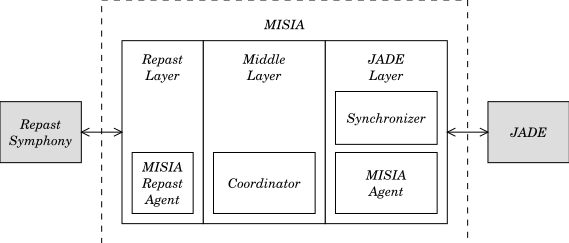
\includegraphics[width=3.0in]{figures/MISIA.pdf}
	\caption{High-level representation of MISIA's architecture (adapted from \cite{garcia2011misia})}
	\label{fig:misia}
\end{figure}

One of the challenges identified by the authors when re-implementing the FIPA interaction protocols was synchronizing them with the Repast tick-based simulation model.
Given JADE's event-driven architecture, MISIA proposes the use of a coordinator agent that informs the JADE-Agent when a tick has passed.
It also proposes its own implementation of the interaction protocols supported by JADE, making them tick-friendly.

%% JREP
\subsection{JRep}
JReps's approach is not as complex as MISIA's.
By having the Repast Simphony agent encapsulate a JADE agent representation, synchronization is immediate and is assured without requiring an external coordinator.
The two agent representations take care of synchronizing any state changes.
Figure \ref{fig:jrep} represents the basic structure of JRep.

\begin{figure}
	\centering
	\includegraphics[width=2.1in]{figures/jrep.pdf}
	\caption{High-level representation of JRep's architecture}
	\label{fig:jrep}
\end{figure}

Each agent takes care of interfacing their respective frameworks. The interaction between agents in JRep is performed using FIPA ACL and the protocol implementations are those provided by the JADE platform. Similarly to MISIA, an Agent Representation Interface is used to introduce the concept of schedule in the JADE agent


%% COMPARISON
\subsection{Comparison with \apiname{}}

JADE is a very rich platform but, for many simulation scenarios, the overhead introduced by it has a significant impact on simulation performance \cite{mengistu2008scalability}. \apiname{}, as we describe with more detail in Section \ref{sec:proposal}, uses an architecture that is conceptually very close to JADE's but tailored for Repast with no extra dependencies. Moreover, the API could be used with other simulation frameworks with little adaptation.

As suggested by Figure \ref{fig:related-repacl}, \apiname{}'s general structure is simpler than that of JRep and MISIA. Our API does not intend to maintain an active connection to a JADE platform, eliminating the need for synchronization. Instead, our goal is to replicate in our API the main features of JADE, allowing for a straightforward and dependency free feature mapping between our API and JADE.

\begin{figure}
	\centering
	\includegraphics[width=2.1in]{figures/repacl.pdf}
	\caption{Basic structure of \apiname{}}
	\label{fig:related-repacl}
\end{figure}

In both MISIA and JRep, even though they attempt to integrate the features from both JADE and Repast, as far as Repast simulations are concerned JADE's multi-threaded infrastructure affects their performance very significantly. The main advantage of our approach is, therefore, the possibility of using Repast with JADE features, namely FIPA specifications including interaction protocols, without the need to interface with JADE. In Section \ref{sec:proposal} we provide a more detailed description of \apiname{}.


%!TEX root = doc.tex
\section{FIPA Specifications} % (fold)
\label{sec:fipa}

% Intro to FIPA in JADE/API
\apiname{} closely follows JADE's architecture regarding the use of protocols and services specified by \gls{FIPA}, represented in Figure \ref{fig:agentManag}. The architecture of the API described in this paper includes four main concepts proposed by \gls{FIPA}: the \gls{DF}, the \gls{MTS}, the \gls{ACL} Message and the Interaction protocols. The following is a brief description of these concepts and of how JADE uses and implements them.

\begin{figure}
	\centering
	\includegraphics[width=2.5in]{figures/agentManag.png}
	\caption{
		Agent Management Reference Model, as specified by FIPA and implemented by JADE. \apiname{} only supports a single Agent Platform.
	}
	\label{fig:agentManag}
\end{figure}

% DF 
The \gls{DF} is a component that provides a yellow page service and is part of the FIPA Agent Management Specification. It allows one agent to perform searches in order to request information about other agents. Only agents that are registered in the DF will be indexed and agents can register and deregister themselves at any time.

% DF Agent Description
When using the DF, agents can specify a series of restrictions that filter the search results. FIPA specifies the DF Agent Description that represents this filter and contains the fields on table \ref{tab:dfAgentDescription}.

\begin{table}
	\normalsize
	\caption{Fields of the DF Agent Description used to filter the results of the DF service.}
	\label{tab:dfAgentDescription}
	\begin{center}
		\begin{tabular}{c|c}
		\hline
		\textbf{Parameter} & \textbf{Description} \\
		\hline
		\texttt{name} & The identifier of the agent \\
		\hline
		\texttt{services} & A list of services supported by this agent \\
		\hline
		\texttt{protocol} & A list of interaction protocols supported by the agent. \\
		\hline
		\texttt{ontology} & A list of ontologies known by the agent. \\
		\hline
		\texttt{language} & A list of content languages known by the agent. \\
		\hline
		\end{tabular}
	\end{center}
\end{table} 

% MTS
The \gls{MTS} is a service, also specified by FIPA, for transportation of ACL messages between agents. It is also responsible for resolving agent addresses, in order to be able to deliver those messages.

% ACL Message
The ACL Message is the envelope that contains the details for communication. \gls{ACL} is specified by \gls{FIPA}, which stipulates what fields the message should contain. Table \ref{tab:fipaACLMessage} was adapted from the FIPA ACL Message structure specification and contains the list of fields in a message. Not all of them are mandatory. FIPA specifies the \texttt{performative} as the only mandatory field, although the \texttt{sender}, \texttt{receiver} and \texttt{content} are usually expected to be present.

\begin{table}
	\normalsize
	\caption{FIPA ACL Message Parameters. The highlighted fields are the ones featured in \apiname{}.}
	\label{tab:fipaACLMessage}
	\begin{center}
		\fboxsep1pt
		\begin{tabular}{c|c}
		\hline
		\textbf{Parameter} & \textbf{Category of Parameters} \\
		\hline
		\colorbox{Apricot}{\texttt{performative}} & Type of communicative acts \\
		\hline
		\colorbox{Apricot}{\texttt{sender}} & \multirow{3}{*}{Participant in communication} \\
		\cline{1-1}
		\colorbox{Apricot}{\texttt{receiver}} \\
		\cline{1-1}
		\texttt{reply-to}  \\
		\hline
		\colorbox{Apricot}{\texttt{content}} & Content of message \\
		\hline
		\texttt{language} & \multirow{3}{*}{Description of Content} \\
		\cline{1-1}
		\texttt{encoding} \\
		\cline{1-1}
		\colorbox{Apricot}{\texttt{ontology}} \\
		\hline
		\colorbox{Apricot}{\texttt{protocol}} & \multirow{5}{*}{Control of conversation} \\
		\cline{1-1}
		\colorbox{Apricot}{\texttt{conversation-id}} \\
		\cline{1-1}
		\texttt{reply-with} \\
		\cline{1-1}
		\texttt{in-reply-to} \\
		\cline{1-1}
		\colorbox{Apricot}{\texttt{reply-by}} \\
		\hline
		\end{tabular}
	\end{center}
\end{table} 

% Behaviors in JADE
JADE uses the concept of behaviours which are adopted by agents that want to play a certain role or perform a task.
Some of these behaviours are meant to be used in agent interaction and include two roles, as specified in FIPA interaction protocols: the initiator and the responder.

%% Implementing these protocols.
In order to create an application using these protocols, programmers only need to extend these behaviours and implement the message handlers.
All the complexity regarding the interaction and networking infrastructure is hidden and taken care of by JADE, allowing the programmer to focus on the implementation of agent behaviour.
%!TEX root = doc.tex
\section{The \apiname{} API} % (fold)
\label{sec:proposal}

%% Intro to the proposal
% Framework limitations issues
The modelling of agent-based systems can be accomplished using on of the wide number of available platforms, such as those surveyed in Nikolai \emph{et al.}\cite{survey}. In order to benefit from different features, modelling the same MAS in different tools may be necessary.
% The main goal of this proposal
The API we propose is the direct result of an undergoing project to solve such necessity. More specifically, we propose a way to easily create JADE-like simulations based solely on the Repast Symphony platform.

The main feature of \apiname{} is the fact that it enables the development of FIPA-compliant MABS in Repast.
% A secondary objective
An objective that has also been taken in consideration in the framework's architecture is ultimately being able to perform a seamless conversion between the two frameworks.
% Conclusion and intro to the section objective
In this section we describe \apiname{}'s architecture thoroughly, while comparing our design decisions with those of JADE.
% [citation needed: is conversion a real need?]


%% Summarizing and comparing Repast and JADE features
%\subsection{Repast and JADE}
% What was missing in Repast?
%JADE and Repast are two popular agent-based frameworks with a very distinct set of features. Table \ref{tab:jadevsrep} summarizes the main differences between the two.

%Our goal is not to reproduce JADE's distributed architecture in Repast. One advantage of using Repast is that, since communication is local (while JADE agents are often spread in different containers), the execution of Repast-based simulations is typically much faster. This also makes it more suited to perform simulations and tests on MAS \cite{mengistu2008scalability} \cite{gormer2011jrep} \cite{garcia2011misia}.

%By incorporating FIPA specifications in Repast, we bring it closer to JADE. Also, when using \apiname{}, programmers that are already comfortable with creating MAS in JADE can feel comfortable enough to produce Repast-based simulations with the features they are used to in JADE.

\subsection{\gls{FIPA} Specifications}

% Brief intro
As previously mentioned, \apiname{} closely follows JADE's architecture and includes the four main concepts proposed by \gls{FIPA}: the \gls{DF}, the \gls{MTS}, the ACL Message and the Interaction protocols.
% The DF Agent Description
Our API implements the DF Agent Description used to filter DF searches. The focus of our tool is the development of local simulations (as opposed to distributed). As such, a single DF exists in each simulation. \apiname{}'s implementation of the MTS is simplified as well due to the absence of a distributed infrastructure; all our agents are local, therefore agent address resolution is unnecessary.

% The Repast Context
It is worth noting that Repast has its own agent manager, named ``Context''.
Repast's Context contains all objects that are to be scheduled. In \apiname{}'s this consists off all active behaviours. 

%\apiname{} offers support to this feature by integrating a reference to the Context in the DF, while preserving the API's independence from Repast. While not present in JADE, this feature was included in \apiname{} out of convenience and is used internally. 

Our implementation uses a version of the ACL Message that is slightly simpler than in the one found in JADE, focusing on the most common elements (the ones highlighted in Table \ref{tab:fipaACLMessage}).

Finally, the main focus of the API we're proposing is the incorporation of \gls{FIPA} Interaction Protocols in Repast. At the present time, we chose to include a few of the most common protocols in \apiname{}, following JADE's implementation.

The \gls{FIPA} protocols from JADE we chose to include in \apiname{} at this point were the ``request-like'' Achieve Rational Effect (AchieveRE) protocol, the Propose protocol and the Contract Net protocol. The AchieveRE is a single protocol that encompasses multiple \gls{FIPA} protocols, namely FIPA-Request, FIPA-query, FIPA-Request-When, FIPA-recruiting and FIPA-brokering protocols, as defined in JADE's documentation \footnote{http://jade.tilab.com/doc/api/jade/proto/AchieveREInitiator.html}.


\subsection{Agent Execution}

In the process of integrating JADE's protocols in \apiname{}, it was necessary to make adaptations to its behaviours' implementation in order to take Repast's concept of time into account. Even though a local application can take advantage of direct method invocation, for the sake of compatibility with JADE communication in \apiname{} is made asynchronously.

JADE agent execution is concurrent and possibly parallel, since JADE supports distributed and multi-threaded agent systems. Agent execution in Repast, on the other hand, in not concurrent. Repast uses a time-share type of execution, granting each agent the right to perform its tasks until they finish them, in sequence, but in no particular order.

Figures \ref{fig:com-example-jade} and \ref{fig:com-example-repast} represent a scenario where two agents send a message to a third one, who then replies to the first two. In Repast, messages are delivered to the agent's mailbox, and processed later on while in JADE, messages can arrive concurrently and be processed right away, because the arrival of a message triggers a correspondent event.

\begin{figure}
	\centering
	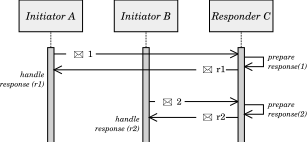
\includegraphics[width=3.0in]{figures/tickExample2.pdf}
	\caption{
		Communication example in JADE. Agents are executed concurrently or in parallel. Agent C tries to handle messages as they arrive and issues the respective reply.
	}
	\label{fig:com-example-jade}
\end{figure}

\begin{figure}
	\centering
	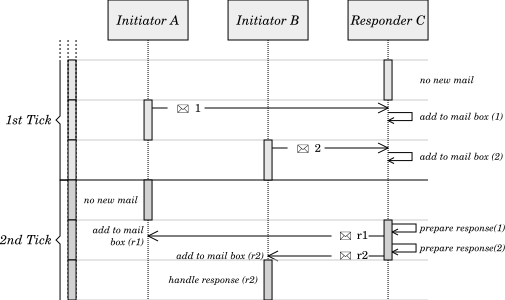
\includegraphics[width=3.5in]{figures/tickExample.pdf}
	\caption{
		Communication example in Repast using \apiname{} in a single tick. In their respective turns, A and B send a message to C, which stays in standby in C's Mailbox. Only in C's turn do these messages get handled.
	}
	\label{fig:com-example-repast}
\end{figure}

It is worth noting that the order by which Repast executes each scheduled behaviour is never guaranteed. In fact, it is not guaranteed that all the behaviours of a single agent are executed together. This is the expected execution when working with Repast as well as with JADE and it is up to the programmer to ensure that the application does not depend on the order or execution.

\subsection{Architecture}

Figure \ref{fig:arch} illustrates the details of \apiname{}'s architecture. Most concepts represented in this diagram are present in JADE, namely the Agent, ACL Message, Behaviour, MTS and DF service.

An agent in \apiname{} contains a set of Behaviours and a Mail Box. The Behaviours have access to the agent who owns them and to its Mail Box. A behaviour tha implements an interaction protocol contains a Message Template which is used in the Mail Box to retrieve relevant messages.

The DF Service, as described before, provides the yellow page service. Agents can register or unregister themselves in the DF as well as perform searches. While tasks can be performed during agent setup, in runtime they are typically executed inside Behaviours.

To follow JADE-like communication, ACL Messages carry agent identifiers (AID) for senders and receivers. These AIDs are returned by the DF as search results and are resolved to an agent by the MTS when sending a message.

The ``plug-in points'' to the API are the Agent and the Behaviour and its derived classes. In Figure \ref{fig:arch}, all protocol definitions are implied by the generic sub-classes ``ProtocolInitiator'' and ``ProtocolResponder''.

\begin{figure}
	\centering
	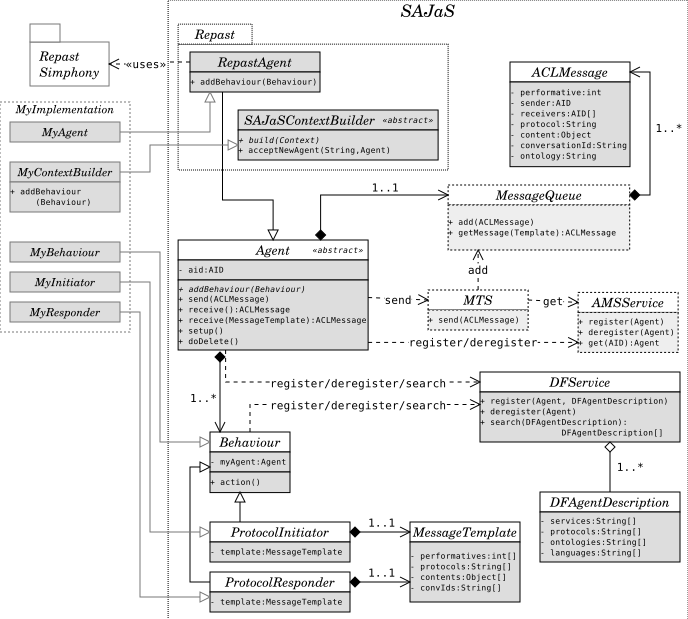
\includegraphics[width=\linewidth]{figures/repacl_arch.pdf}
	\caption{Detailed architecture or \apiname{}}
	\label{fig:arch}
\end{figure}

\subsection{Using Repast}

The Context is an utility created to provide support for Repast. In order for the simulation to run, scheduled behaviours must be added to it. In Repast simulations, the context must be set in the API by the Context Builder, which functions as the main class of a Repast simulation. We decided to integrate this feature in \apiname{} despite not being present in JADE to preserve the API's independence from Repast. This way, \apiname{} has it's own internal representation of the context.

Repast uses Java annotations to indicate which methods are to be scheduled. \apiname{}'s Behaviours contain an \texttt{action} method that should be scheduled and called when programmers implement their own instances of the Behaviours in the API. The following Java snippet represents the basic recommended usages of the Repast scheduler when extending \apiname{}'s Behaviours. Being a Repast construct, the action method is not used for actual behaviour tasks.

\begin{lstlisting}[language=Java]
	public class MyBehaviour extends Behaviour {
		...
		@Override
		@ScheduledMethod(start=1, interval=0.1)
		public void action() {
			super.action();
		}
		...
	}
\end{lstlisting}


% section proposal (end)
%!TEX root = doc.tex
\section{Verification}
\label{sec:verification}

TODO:

  - Finish protocols implementation (ideally, at least contract net)

  - Create test with multiple agents (dozens)

  - Create Repast interface to show agent interaction à lá JADE sniffer

%!TEX root = doc.tex
\section{Future Work}
\label{sec:prototype}

In this section we specify some of the future developments that are planned for \apiname. We also present the tool under development that initially created the need for the development of \apiname.

\subsection{Conversion Tool Prototype}

The goal of the tool we propose is to allow the automatic conversion of Repast simulations into JADE applications. This conversion tool will not only allow the developer to quickly generate a MAS or create a simulation but also enables a proficient programmer in one framework to quickly get started in developing with the other framework. Figure \ref{fig:prototypeFlow} illustrates these two plausible workflows.

\begin{figure}[h]
	\centering
	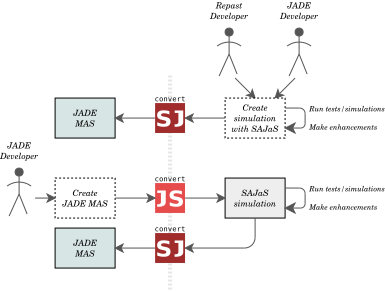
\includegraphics[width=3.0in]{figures/prototypeFlow.pdf}
	\caption{
		Two possible workflows for \apiname{} users
	}
	\label{fig:prototypeFlow}
\end{figure}

The code conversion tool uses the Java Development Tools (JDT) from Eclipse which enables Java programmers to perform introspection and reflection tasks with ease. This approach allows programmers to perform code transformations without having to create parsers for Java code and abstract syntax trees (AST).

The conversion tool will be developed in the form of an Eclipse plug-in, in order to be able to make use of all JDT features.

\subsection{\apiname{} development}

Although \apiname{} is already fit for development of Repast simulations, it's still an ongoing project. One important trait of \apiname{} is that, although tailored for repast, it's very generic. This means that MABS built using other Java simulation tools can integrate our API successfully in the future and, therefore, use Jade-based tools.

%!TEX root = .\doc.tex
\section{Conclusion}
\label{sec:conclusion}

The development of MAS may require the use of tools that are not readily available in the agent-based framework originally chosen. The API architecture we propose in this paper emerges as a need to solve a concrete instance of this problem. \apiname{} is our solution to integrating FIPA specifications in MABS frameworks, more specifically Repast, as well as allowing the creation of JADE-based simulations.

The goal of our API is not only to enrich Repast and other simulation frameworks, but also to allow proficient JADE developers in quickly getting started in developing simulations using familiar JADE-based tools. \apiname{} also opens the door to MAS to MABS conversion.

The short experiment we described in the previous section showed that our API is capable of handling simulations with a large number of agents, which is common in many simulation scenarios. Aside from the inherent advantages of using open standards in agent systems, \apiname{}'s JADE-based architecture brings Repast closer to JADE. The immediate result of this architecture is that converting models built with Repast using \apiname{} into JADE MAS is very straightforward.


%\bibliographystyle{llncs}
%\bibliography{IEEEabrv, references}
%\bibliographystyle{splncs}
%\bibliographystyle{spbasic}
\bibliographystyle{plain}
\bibliography{references}


\end{document}

